\documentclass{report}

\usepackage[english]{babel}
\usepackage[letterpaper,top=2cm,bottom=2cm,left=3cm,right=3cm,marginparwidth=1.75cm]{geometry}
\usepackage{amsmath}
\usepackage{graphicx}
\usepackage[colorlinks=true, allcolors=blue]{hyperref}
\graphicspath{{images/}}
\setcounter{tocdepth}{4}
\setcounter{secnumdepth}{4}
\usepackage{varwidth}
\usepackage{verbatim}
\usepackage{pdfpages}


\title{Using GPLK to solve Mixed Integer Programming (MIP) Linear Optimization Models}

\author{Mr Ashlin Darius Govindasamy\\ \large{University of South Africa}}

\date{\today}

\begin{document}
\maketitle
\newpage

% create centered abstract
\begin{abstract}
    This paper is a guide to using the Octave programming language and module (GPLK)  to solve linear optimization models.
\end{abstract}



\tableofcontents

%for adding page numbers
\pagenumbering{arabic} 


%add more chapters like this
\chapter{GPLK Parameters and Flags}
%add subsections like this
\subsection{Introduction}
Octave can solve Linear Programming problems using the glpk function. That is, Octave can solve

\newenvironment{centerverbatim}{%
  \par
  \centering
  \varwidth{\linewidth}%
  \verbatim
}{%
  \endverbatim
  \endvarwidth
  \par
}

\begin{verbatim}
min C'*x
\end{verbatim}

subject to the linear constraints
\begin{equation}
A*x = b \;\;\;\; \text{where} \; x \geq 0
\end{equation}

the \textbf{glpk} function also supports variations of this problem.

\subsection{Syntax}
\begin{verbatim}
    : [xopt, fmin, errnum, extra] = glpk (c, A, b, lb, ub, ctype, vartype, sense, param)
\end{verbatim}

Given 3 Parameters, \textbf{gplk} solves the following standard form linear programming problem:

\begin{equation}
\begin{aligned}
\min & \; c^T x \\
\text{subject to} & \; A x = b \\
x \geq 0
\end{aligned}
\end{equation}

but it can also solve the following variations of this problem:

% center code
\begin{centerverbatim}
[min|max] c'*x
\end{centerverbatim}

subject to the linear constraints
\begin{centerverbatim}
    A*x [ "=" | "<=" | ">=" ] b
    x >= LB
    x <= UB
\end{centerverbatim}

\subsection{Parameters and Flags}
 
%inject .pdf
\setboolean{@twoside}{false}
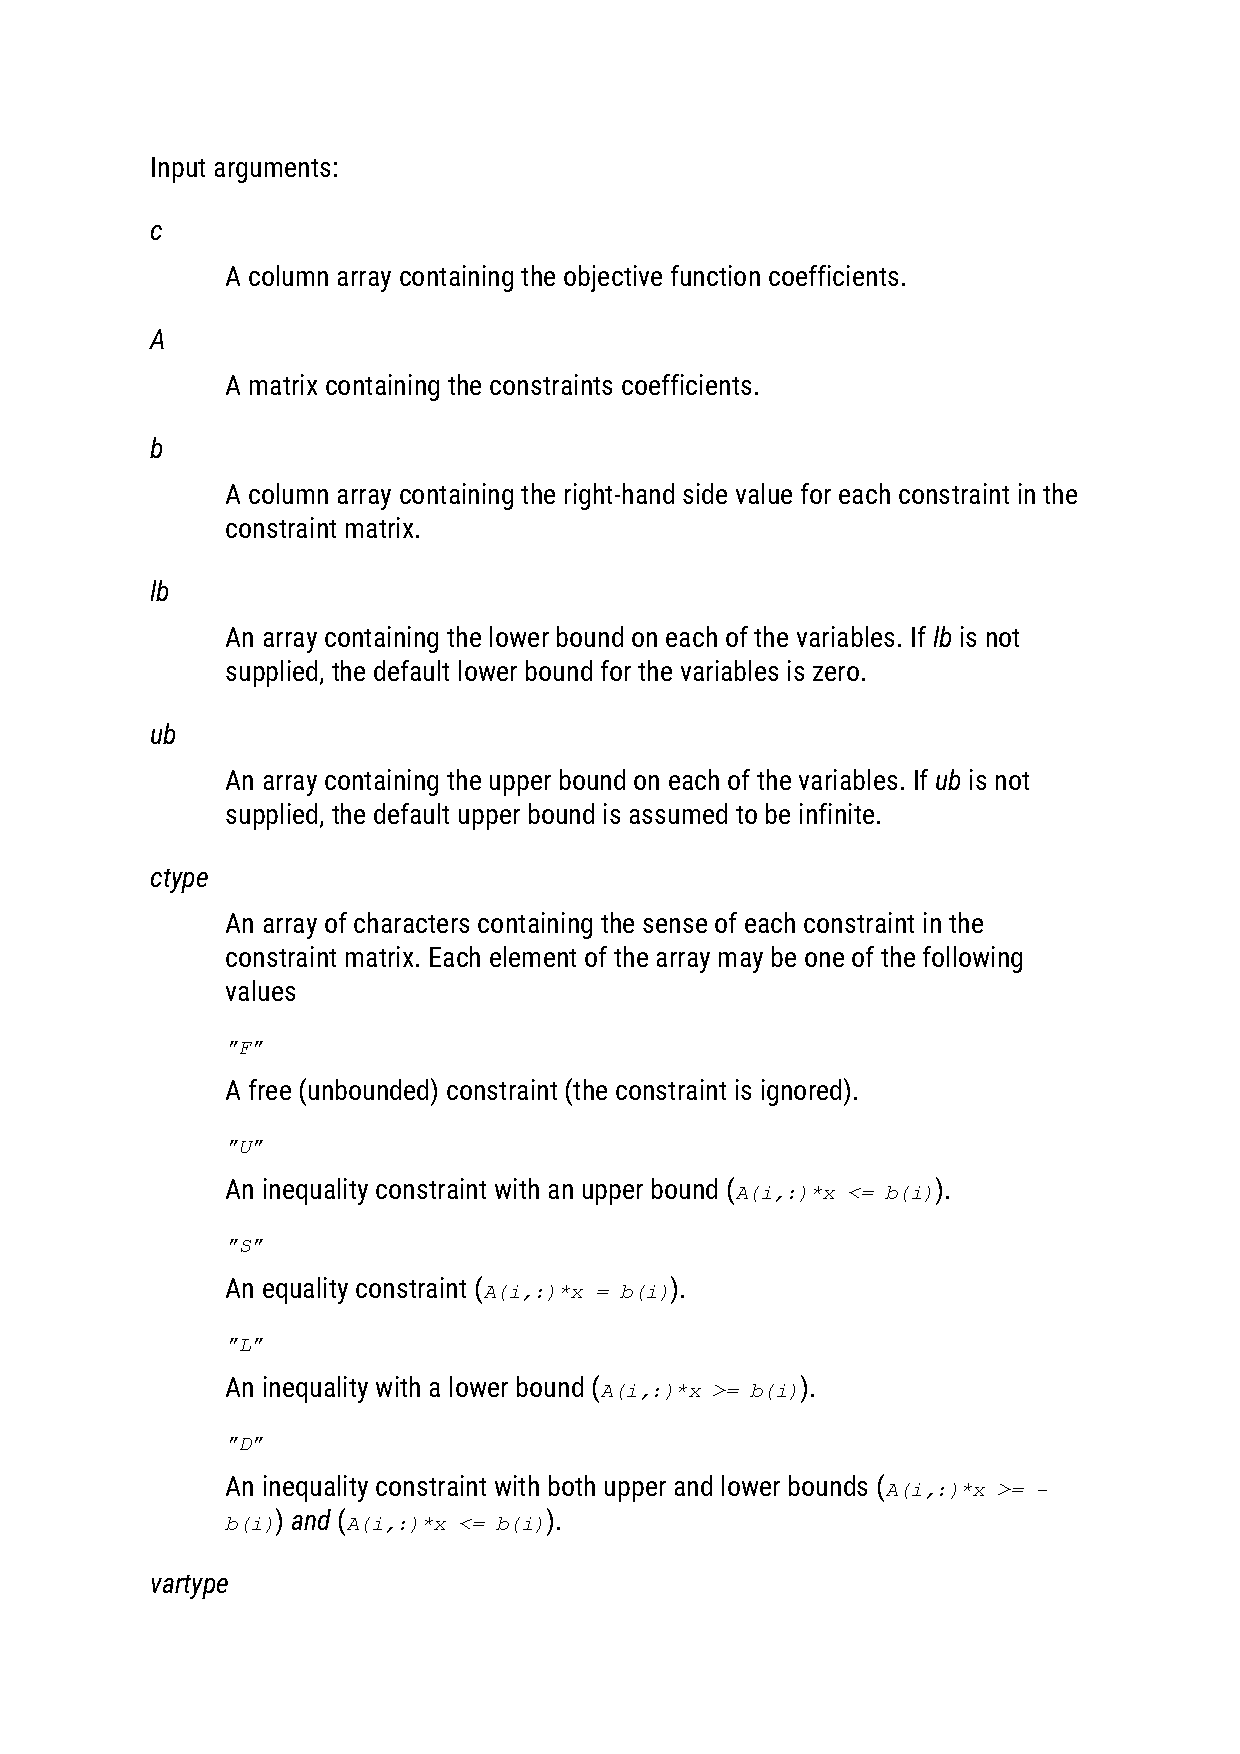
\includepdf[pages=-]{chapters/manual.pdf}

\chapter{Implementation and Examples}
\subsection{Implementation and Examples}

\subsubsection{Example 1: Minimizing Optimization Multiple Integer Programming Problem}

Consider the following optimization problem:

\begin{equation}
\begin{aligned}
    L = & \; 2x_1 + 3x_2 + 4x_3 + 5x_4 \\
    \text{subject to} & \; 2x_1 + 3x_2 + 4x_3 + 5x_4 \leq 100 \\
    & \; 6x_1 + 3x_2 + 7x_3 + 3x_4 \geq 50 \\
    & \; x_1 + x_2 + x_3 + x_4 \leq 10 \\
    & \; x_1 + x_2 + x_3 + x_4 \geq 5 \\
    & \; x_1 \geq 0 \\
\end{aligned}
\end{equation}

The Upper Bound Symbol is \(\leq\) and the Lower Bound Symbol is \(\geq\) \\

We can solve this problem using the \textbf{glpk} function in Octave. The \textbf{glpk} function takes 9 parameters. The first 5 parameters are the objective function, the linear constraints, the lower bound and the upper bound. The last 4 parameters are the constraint type, the variable type, the sense and the parameters.

\begin{equation}
\begin{aligned}
    \text{glpk} (c, A, b, lb, ub, ctype, vartype, sense, param)
\end{aligned}
\end{equation}

Lets find our solution using Octave:

\begin{equation}
C =
    \begin{bmatrix}
        2 \\
        3 \\
        4 \\
        5 \\
    \end{bmatrix}
\end{equation}

C is the objective function. The objective function is the function we want to minimize or maximize. In this case we want to minimize the objective function.

\begin{equation}
A = 
\begin{bmatrix}
    2 & 3 & 4 & 5 \\
    6 & 3 & 7 & 3 \\
    1 & 1 & 1 & 1 \\
    1 & 1 & 1 & 1 \\
    1 & 0 & 0 & 0 
\end{bmatrix}
\end{equation}

A is the matrix of the linear constraints. The linear constraints are the constraints that the variables must satisfy. In this case we have 5 linear constraints.

\begin{equation}
b =\begin{bmatrix}
    100 \\
    50 \\
    10 \\
    5 \\
    0
\end{bmatrix}
\end{equation}

b is the matrix of the linear constraints. The linear constraints are the constraints that the variables must satisfy. In this case we have 5 linear constraints.

\begin{equation}
lb = \begin{bmatrix}
    0 \\
    0 \\
    0 \\
    0
\end{bmatrix}
\end{equation}

lb is the lower bound matrix. The lower bound matrix is the matrix of the lower bounds of the variables. In this case we have 4 variables and we have no lower bounds.

\begin{equation}
ub = \begin{bmatrix}
    \infty  \\
    \infty  \\
    \infty  \\
    \infty 
\end{bmatrix}
\end{equation}

ub is the upper bound matrix. The upper bound matrix is the matrix of the upper bounds of the variables. In this case we have 4 variables and we have no upper bounds.

\begin{equation}
ctype = \begin{bmatrix}
    'U' \\
    'L' \\
    'U' \\
    'L' \\
    'L'
\end{bmatrix}
\end{equation}

ctype is the constraint type matrix. The constraint type matrix is the matrix of the constraint types. In this case we have 5 constraints and we have 2 upper bounds, 2 lower bounds and 1 equality constraint.

\begin{equation}
vartype = \begin{bmatrix}
    'C' \\
    'C' \\
    'C' \\
    'C'
\end{bmatrix}
\end{equation}

vartype is the variable type matrix. The variable type matrix is the matrix of the variable types. In this case we have 4 variables and we have 4 continuous variables.

\begin{equation}
sense = -1
\end{equation}

sense is the sense of the optimization problem. The sense of the optimization problem is the sense of the objective function. In this case we want to minimize the objective function so we set the sense to -1.

We set our parameters to
\begin{verbatim}
    param.msglev = 1;
\end{verbatim}

Msglev is the message level. The message level is the level of the messages that are displayed. In this case we set the message level to 1 so that we can see the messages.

Now we can implement our octave code

\begin{verbatim}
c = [2; 3; 4; 5];
A = [2 3 4 5; 6 3 7 3; 1 1 1 1; 1 1 1 1; 1 0 0 0];
b = [100; 50; 10; 5; 0];
lb = [0; 0; 0; 0];
ub = [inf; inf; inf; inf];
ctype = ['U'; 'L'; 'U'; 'L'; 'L'];
vartype = ['C'; 'C'; 'C'; 'C'];
sense = 1;
param.msglev = 1;
[x, fmin, status, extra] = glpk (c, A, b, lb, ub, ctype, vartype, sense, param)
\end{verbatim}

When we run this code we get the following output:

\begin{verbatim}
    x =

    8.3333
         0
         0
         0
 
 fmin = 16.667
 status = 0
 extra =
 
   scalar structure containing the fields:
 
     lambda =
 
             0
        0.3333
             0
             0
             0
 
     redcosts =
 
             0
        2.0000
        1.6667
        4.0000
 
     time = 0
     status = 5
\end{verbatim}

In conclusion we solved the question for the most optimized minimal variables we should use
\begin{equation}
\begin{aligned}
    x_1 = 8.3333 \\
    x_2 = 0 \\
    x_3 = 0 \\
    x_4 = 0
\end{aligned}
\end{equation}

To get our objective function to be minimized to 16.667

\subsubsection{Example 2: Real World Example}
ADGSTUDIOS manufactures two types of wooden toys: peace-keepers and trains. A peace-keeper sells for R27 and uses R10 worth of raw materials. Each peace-keeper that is manufactured increases ADGSTUDIOS's variable labour and overhead costs by R14. A train sells for R21 and uses R9 worth of raw materials. Each train built increases ADGSTUDIOS's variable labour and overhead costs by R10. The manufacture of wooden peace-keeper and trains requires two types of skilled labor: carpentry and finishing. A peace-keeper requires 2 hours of finishing labour and 1 hour of carpentry labour. A train requires 1 hour of finishing labour and 1 hour of carpentry labour. Each week, ADGSTUDIOS can obtain all the needed raw material but only 100 finishing hours and 80 carpentry hours. Demand for trains is unlimited, but at most 40 peace-keepers are bought each week. ADGSTUDIOS wants to maximize weekly profit (revenues-costs).

\begin{equation}
\begin{aligned}
    \text{maximize} \; & (27-10-14)x_1 + (21-9-10)x_2 \\
    \text{subject to} \; & 10x_1 + 9x_2 \leq 100 \\
    & 2x_1 + x_2 \leq 80 \\
    & x_1 \leq 40 \\
    & x_1, x_2 \geq 0
\end{aligned}
\end{equation}

Our objective function is
\begin{equation}
\begin{aligned}
    C = 3x_1 + 2x_2
\end{aligned}
\end{equation}

Octave code

\begin{verbatim}
c=[3 2]; % maximise z = 3 x_1 + 2 x_2
% subject to:
A=[2,1;1,1;1,0;1,0;0,1]; % coefficients
b=[100;80;40;0;0] % bounds

lb=[0;0]
ub=[Inf;Inf];
ctype = ["U";"U";"U";"L";"L"]; % indicates upper bound or lower bound
vtype = ["C";"C"]; % continuous variables

sense=-1; % maximises
[xopt,zmx]=glpk(c,A,b,lb,ub,ctype,vtype,sense)
\end{verbatim}

Output

\begin{verbatim}
xopt =
    20
    60

zmx = 180
\end{verbatim}

Our optimal solution is
\begin{equation}
\begin{aligned}
    x_1 = 20 \\
    x_2 = 60
\end{aligned}
\end{equation}

So maximum revenue for ADGSTUDIOS is R180 each week. The report also shows that ADGSTUDIOS can maximize weekly profit by producing 20 peace-keepers and 60 trains each week.



\newpage

\end{document}
